%% pdflatex
\documentclass[10pt]{beamer}
%% \usepackage{upgreek}
\usepackage{hyperref}
%% Fonts
\usepackage{multicol}
\usepackage{mathabx}
\usepackage[scaled]{helvet}
\usepackage{lmodern}
\usepackage{fancybox}
\usepackage{eulervm}
\usefonttheme[onlymath]{serif}
\usefonttheme{professionalfonts}
\usefonttheme{structurebold}
\hypersetup{backref}
\usepackage{bm}
%% Color & Theme
\definecolor{SUblue}{RGB}{0,0,180}
\usecolortheme[RGB={0,0,180}]{structure}
\usetheme{Boadilla}
\setbeamertemplate{navigation symbols}{}
\setbeamerfont{title}{size=\large}
\setbeamerfont{frametitle}{size=\large}
\setbeamerfont{framesubtitle}{size=\large, shape =$\color{violet}{\looparrowdownright}~$}
\setbeamercolor{title}{fg=white, bg= SUblue!75!green}
\setbeamercolor{framesubtitle}{fg=violet}


\hypersetup{
colorlinks=true}

\title[Teaching R]{{\textbf{Teaching R as a general programming language}}}

% \author[Feng Li]{\\\vspace{0.7cm}\textbf{Feng Li}  \\\vspace{0.2cm}
%   \textbf{\footnotesize{(jointly with Mattias Villani)}}}
\vspace{2cm}
\author[Feng Li]{\\ \textbf{Feng Li}}

\institute[Stockholm University]{\footnotesize{\textbf{Department of
      Statistics, Stockholm University}}}
\date{\color{SUblue}{ \textbf{Nov, 2012}}}

\begin{document}
%% Title page

\begin{frame}[plain]
  \titlepage

\end{frame}


%%%%%%%%%%%%%%%%%%%%%%%%%%%%%%%%%%%%%%%%%%%%%%%%%%%%%%%%%%%%%%%%%%%%%%%%%%%%%%
\section{Introduction and background}

\begin{frame}
  \frametitle{Introduction and background}
  \begin{itemize}

  \item Intended learning outcomes
    \begin{itemize}
    \item Know the general programming logic
    \item Know the idea of object-oriented programming
    \item Use R as a daily tool: a better version of calculator/Excel

    \end{itemize}

  \item Course book
    \begin{itemize}
    \item  Many books available, most focus on implementing statistical
      methods/graphics in R.
    \item \textbf{R Cookbook} by Paul Teetor
    \end{itemize}

  \item Teaching activities
    \begin{itemize}
    \item Lectures: Materials available at
      \texttt{\url{http://www.mattiasvillani.com/teaching/programming-in-r/}}
    \item Labs: R on Solaris machine
      \\We design questions for the students (some examples later).
    \end{itemize}
  \end{itemize}
\end{frame}


\begin{frame}
  \frametitle{Course covered topics}
  \begin{itemize}
  \item R workspace: \\\texttt{ls(), rm(), getwd(), setwd(), save.image(), load(), source()}
  \item Data structures and manipulation:
    \\\texttt{vector(), matrix(), array(), data.frame(), list()}
    \\\texttt{read.table(), [ ], [[ ]], \$}

  \item Object-oriented programming: \\\texttt{ class(), typeof(), function(), return()}
  \item Loops and \texttt{if else} condition
  \item Vectorization: \texttt{*apply()}
  \item Basic graphical tools: \texttt{plot()}, \texttt{lines()}, \texttt{par()}
  \item Simple debugging tools: \texttt{print(), browser(), traceback()}
  \item Packages, helps and documentations.
  \item Introduction to statistical tests and linear regression model with R.
  \item Good programming style: \\\texttt{readability (commenting, naming)}, \texttt{extendability}
  \end{itemize}
\end{frame}


\begin{frame}
  \frametitle{Sample lab questions}
  \framesubtitle{Roots for quadratic equation}
  \begin{figure}
    \centering
    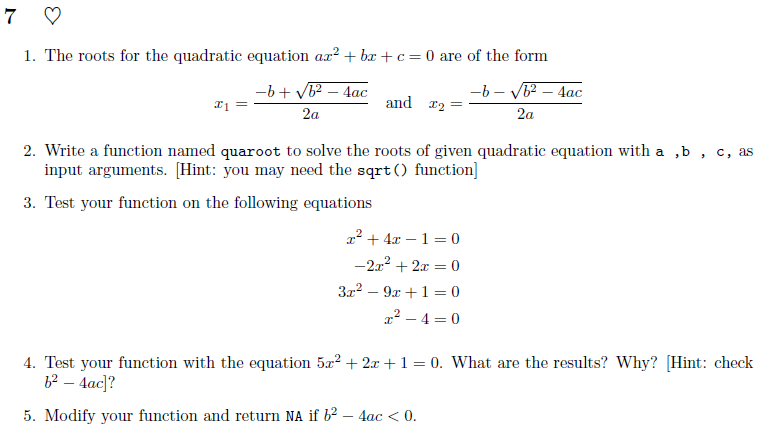
\includegraphics[width=0.9\textwidth]{quaroot}
  \end{figure}
\end{frame}


\begin{frame}
  \frametitle{Sample lab questions}
  \framesubtitle{Factorial function (1)}
  \begin{figure}
    \centering
    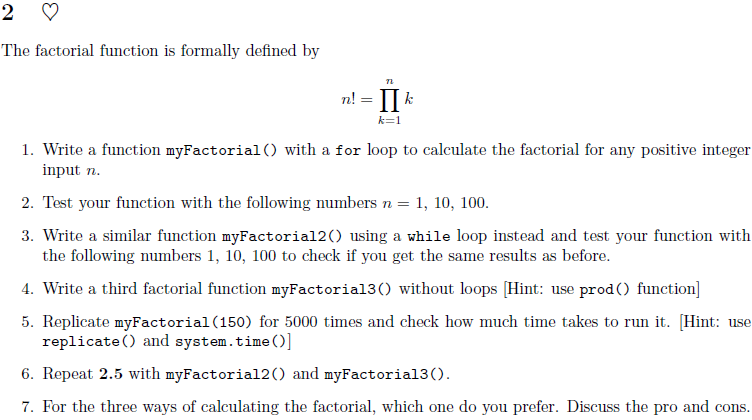
\includegraphics[width=0.9\textwidth]{prod1}
  \end{figure}
\end{frame}


\begin{frame}
  \frametitle{Sample lab questions}
  \framesubtitle{Factorial function (2)}
  \begin{figure}
    \centering
    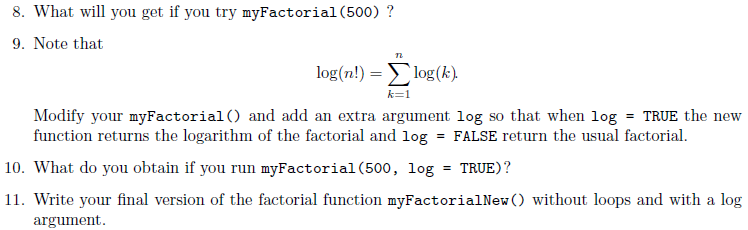
\includegraphics[width=0.9\textwidth]{prod2}
  \end{figure}
\end{frame}


\begin{frame}
  \frametitle{Sample lab questions}
  \framesubtitle{Debug a function}
  \begin{figure}
    \centering
    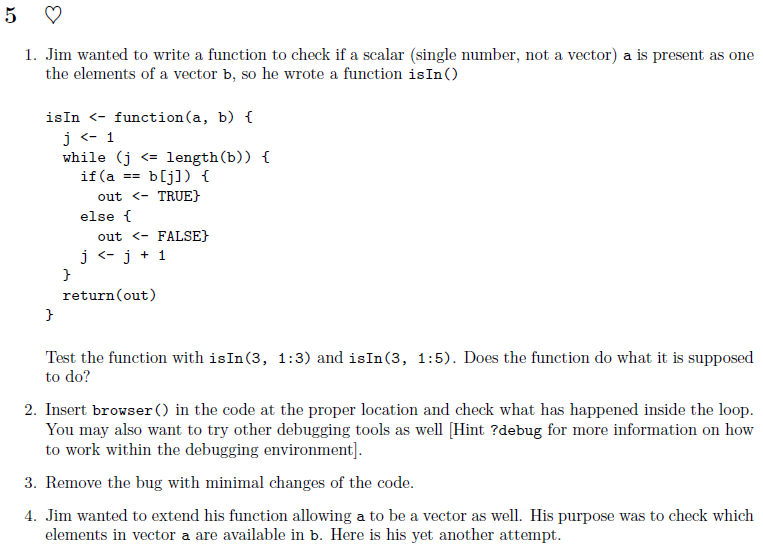
\includegraphics[width=0.9\textwidth]{debug}
  \end{figure}
\end{frame}


\begin{frame}
  \frametitle{Sample lab questions}
  \framesubtitle{Write efficient code}
  \begin{figure}
    \centering
    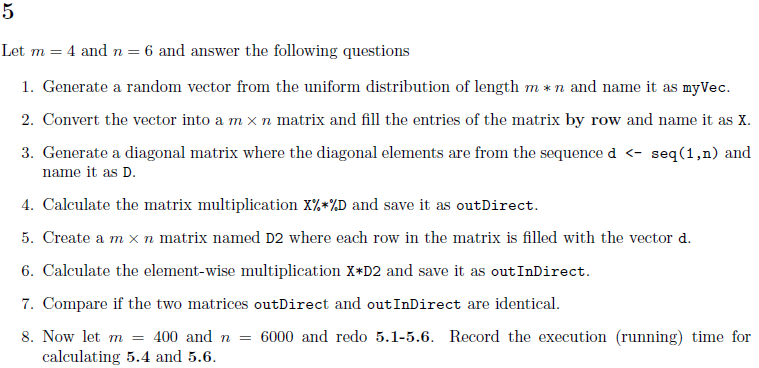
\includegraphics[width=0.9\textwidth]{matrix}
  \end{figure}
\end{frame}


\begin{frame}[plain]
  \addtocounter{framenumber}{-1}
  \begin{center}
    \begin{figure}
      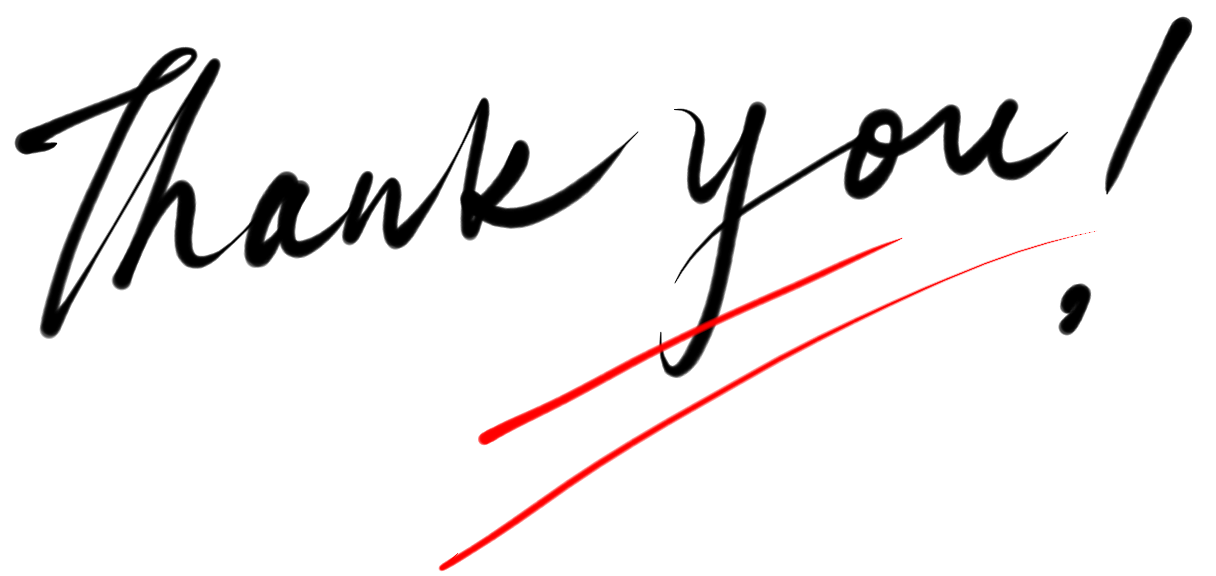
\includegraphics[height=3.0cm]{thankyou}
    \end{figure}
  \end{center}


\begin{itemize}
\item [$\circ$] Questions?
\item [$\circ$] Contact: Feng Li,
  \texttt{\color{purple}{<feng.li@stat.su.se>}}.%, \texttt{\color{purple}{http://feng.li/}}
\end{itemize}

\end{frame}



\end{document}